\documentclass[
../../EiKI_Summary.tex,
]
{subfiles}
    
\externaldocument[ext:]{../../EiKI_Summary.tex}
% Set Graphics Path, so pictures load correctly
\graphicspath{{../../}}

\begin{document}
\section{Constraint Satisfaction Problems}
\begin{defbox}
    [Constraint Satisfaction Problem]
    \defc{Constraint Satisfaction} is a technique where a problem is solved when its solution satisfies certain constraints or rules of the problem.
\end{defbox}

\defc{Components}:
\begin{itemize}
    \item A state, defined by \defc{variables $X_i$} with \defc{d} values from \defc{domain $D_i$}
    \item A goal test, defined as a set of \defc{constraints $C$} specifying allowable combinations of values for subsets of variables.
\end{itemize}

\defc{Solving Constraint Satisfaction Problems}:
\begin{itemize}
    \item A state space
    \item Notion of the solution
\end{itemize}

\begin{figure}
    [H]
    \centering
    \caption{Example of a Constraint Satisfaction Problem}
    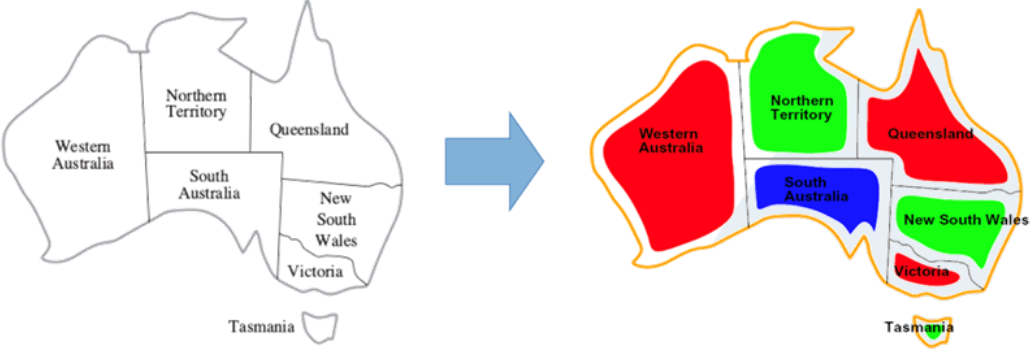
\includegraphics[width=0.6\textwidth]{Pics/05/ConstraintSatisfactionProblemEx.png}
\end{figure}
\textbf{Problem:} Assign each territory a colour such that no two adjacent territories have the same colour.

\textbf{Variables:} $X = \{WA, NT,Q,NSW,V,SA,T\}$\\
\textbf{Domain of Variables:} $D = \{red, green, blue\}$\\
\textbf{Constraints:} $C = \{SA \not= WA, SA \not= NT, SA \not=Q,\dots\}$

\subsection{Assignment of Values to Variables}
A state in state-space is not a ''blackbox'' as in standard search, but defined by assigning values to some or all variables.

\begin{csmb*}
    $X_1 = v_1, X_2 = v_2, \dots, X_d = v_d$
\end{csmb*}

The assignment of these values can be done in different ways:
\begin{enumerate}
    \item \defc{Consistent/Legal Assignment}: An assignment is consistent if it satisfies all constraints or rules.
    \item \defc{Complete Assignment:} An assignment is complete if every variable is assigned a value, and the solution to the CSP remains consistent.
    \item \defc{Partial Assignment:} An assignment is partial if some variables are not assigned values.
\end{enumerate}

\subsection{Constraint Graphs}
Constraint Graphs are often constructed because abstraction of the problem makes it easier to solve and understand.

A constraint graph is usually denoted with
\begin{itemize}
    \item Every variable is represented by a node
    \item Every edge indicates a constraint between two variables
\end{itemize}

\begin{figure}
    [H]
    \centering
    \caption{Example of a Constraint Graph}
    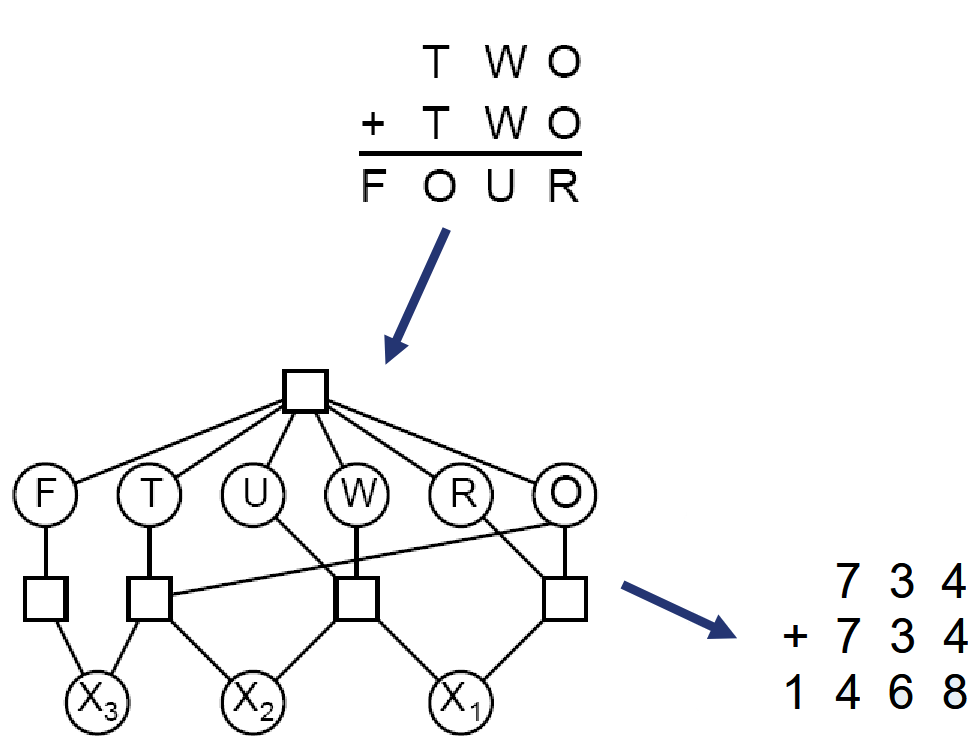
\includegraphics[width=0.4\textwidth]{Pics/05/ConstraintGraphEx.png}
\end{figure}

\textbf{Problem:} Assign uniques value to the variables of each letter, so that resulting equation is true. \\

\textbf{Variables:} $X = \{T,W,O,F,U,R\}$\\
\textbf{Domain of Variables:} $D = \{0,1,2,3,4,5,6,7,8,9\}$\\
\textbf{Constraints:} $C = \{T \not = W \not= O \not= F \not= U \not= R\}$\\
$\cup$ \inlcodebox{$\texttt{int}(''T''+''W''+''O'') + \texttt{int}(''T''+''W''+''O'') = \texttt{int}(''F''+''O''+''U''+''R'')$}

Here the connected nodes are involved in (in-)equations:

\begin{csmb*}
    $\begin{array}{r c l}
        2\cdot O &=& 10 \cdot X_1 + R \\
        2\cdot W + X_1 &=& 10 \cdot X_2 + U \\
        2\cdot T + X_2 &=& 10 \cdot X_3 + O \\
        F &=& X_3 \\
        T \not= W \not= O &\not=& F \not= U \not= R
    \end{array}
    $
\end{csmb*}

\subsection{Types of Constraints}
\begin{itemize}
    \item \defc{Unary constraints:} Involve a single variable (e.g. South Australia $\not=$ green)
    \item \defc{Binary constraints:} Involve two variables (e.g. South Australia $\not=$ Wester Australia)
    \item \defc{Higher-order constraints:} Involve more than two variables (e.g. $2\cdot W + X_1 = 10 \cdot X_2 + U$)
\end{itemize}

\defc{Preferences / Soft constraints:} 
\begin{itemize}
    \item Not binding, but should be considered during search 
    \subitem $\rightarrow$ Constrained optimization problems
    \item e.g. Red is better than green
\end{itemize}

\subsection{Solving CSPs: Search}
\defc{Basic Idea:}
\begin{enumerate}
    \item Successively assign values to variable
    \item Check constraints
    \item If constraint is violated $\rightarrow$ backtrack
    \item Repeat until all variables have assigned values that satisfy constraints
\end{enumerate}

To do this we map CSPs into search problems:
\begin{itemize}
    \item Nodes = assignments of values to a subset of the variables
    \item Neighbors of a node = nodes in which values are assigned to one additional variable
    \item Start node = empty assignment
    \item Goal node = a node which assigns a value to each variable and satisfies all constraints
\end{itemize}

\subsubsection{Naive Search}
Naive Search is practically a \textbf{brute-force} method. It systematically explores all possible assignments of v values to n variables. This, of course, is incredibly innefficient and results in exponential time complexity. The number of leaves in the search tree grows with $n!v^n$.

\subsubsection{Backtracking Search}
\defc{Basic Idea:}
As assignments are commutative ([WA = red then NT = green] = [Nt = green then WA = red]) we can reduce the number of leaves in the search tree by only considering nodes that have not been visited before.

\begin{codebox}
    [Backtracking Algorithm]
    \begin{algorithm}[H]
        \SetKwFunction{backtracks}{backtrack\_search}
        \SetKwFunction{recbacktrack}{recursive\_backtrack}
        \SetKwFunction{gunva}{get\_unassigned\_variable}
        \SetKwFunction{getva}{get\_variables}
        \SetKwFunction{ordova}{order\_domain\_values}
        \SetKwFunction{constraints}{constraints}
        \SetKwFunction{iscompl}{is\_complete}
        \SetKwFunction{adddd}{add}
        \SetKwFunction{removee}{remove}

        \Fn{\backtracks{csp}}{
            \KwRet \recbacktrack{csp, \{\}}\;
        }
        \Fn{\recbacktrack{csp, assignment}}{
            \If{\iscompl{assignment}}{
                \KwRet assignment\;
            }
            var = \gunva{\getva{csp}, assignment, csp}\;
            \ForEach{value in \ordova{var, assignment, csp}}{
                \If{value is consistent with assignment given \constraints{csp}}{
                    assignment.\adddd{\{var = value\}}\;
                    result = \recbacktrack{csp, assignment}\;
                    \If{result != failure}{
                        \KwRet result\;
                    }
                    assignment.\removee{\{var = value\}}\;
                }
            }
            \KwRet failure\;
        }
    \end{algorithm}
\end{codebox}

This is still not ideal as in the worst case the complexity is still exponential. This can be improved by including heuristics.

\newpage
\subsection{Heuristics for CSPs}
\begin{itemize}
    \item \defc{Domain-Specific Heuristics:} Depend on the particular characteristics of the problem.
    \item \defc{General-Purpose Heuristics:} Can work on any CSP.
    \begin{itemize}
        \item \textbf{Minimum Remaining Value:} Choose variable with fewest consistent values
        \begin{figure}
            [H]
            \centering
            
\includegraphics[width=0.6\textwidth]{Pics/05/MinimumRemainingValuesHeuristic.png}
        \end{figure}
        \item \textbf{Degree Heuristic:} Choose variable with the most constraints on remaining variables
        \begin{figure}
            [H]
            \centering
            
\includegraphics[width=0.6\textwidth]{Pics/05/DegreeHeuristic.png}
        \end{figure}
        \item \textbf{Least Constraining Value Heuristic:} Given a variable, choose the value that rules out the fewest values in the remaining variables
        \begin{figure}
            [H]
            \centering
            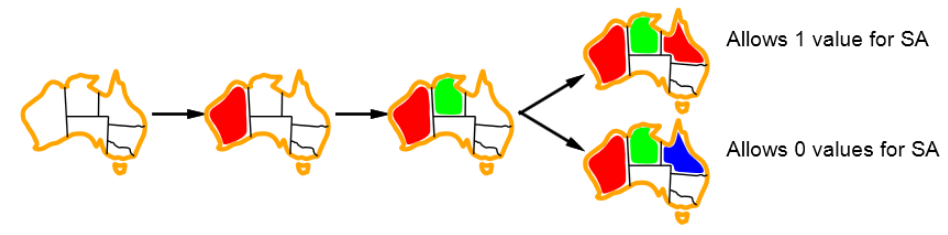
\includegraphics[width=0.8\textwidth]{Pics/05/LeastConstrainingValueHeuristic.png}
        \end{figure}
    \end{itemize}
\end{itemize}

If utilized in this order, these heuristics will greatly improve search speed.

\subsection{Constraint Propagation}
\begin{defbox}
    [Node Consistency]
    A variable (node) is consistent if the possible values of this variable are conform to all unary constraints.
\end{defbox}

\begin{defbox}
    [Local Consistency]
    Local consistency is defined by a graph where each of its nodes is consistent with its neighbors. This is done by iteratively enforcing the constraint corresponding to the edges.
\end{defbox}

\begin{defbox}
    [Arc]
    A constraint involving two variables is called an \defc{arc} or binary constraint.
\end{defbox}

\begin{defbox}
    [Arc Consistency]
    An arc is consistent if for each value of $X$ in the domain of $X$ there exists a value $Y$ in the domain of $Y$ such that the constraint $\text{arc}(X, Y)$ is satisfied.

    \begin{csmb*}
        $\forall X \in \text{dom}(X), \exists Y \in \text{dom}(Y): \text{arc}(X, Y) \text{ is satisfied}$
    \end{csmb*}
\end{defbox}

\subsubsection{Forward Checking}
\defc{Basic Idea:}
Keep track of remaining legal values for unassigned variables and terminate search, when any variable has no legal values left.

\begin{figure}
    [H]
    \centering
    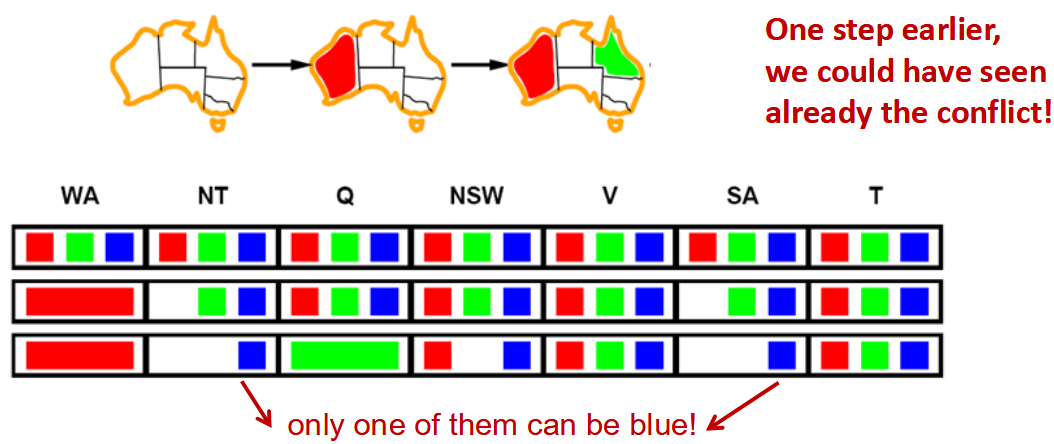
\includegraphics[width=0.6\textwidth]{Pics/05/ForwardChecking.png}
\end{figure}

\subsubsection{Maintainting Arc Consistency (MAC)}
After each assignment of a value to a variable, possible values of the neighbors have to be updated.

\begin{figure}
    [H]
    \centering
    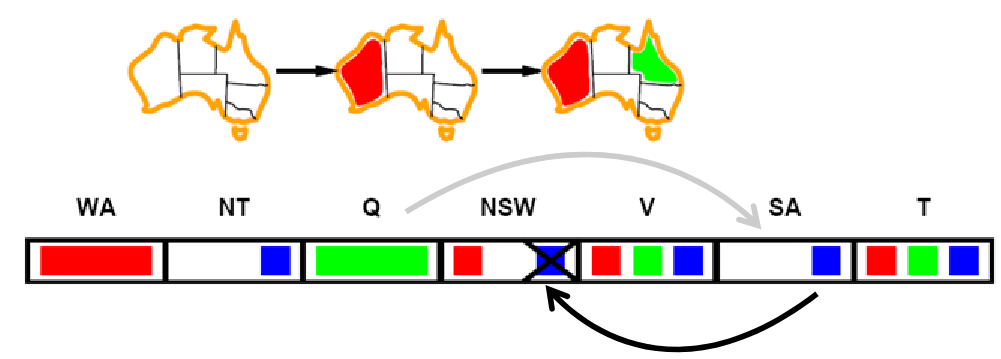
\includegraphics[width=0.6\textwidth]{Pics/05/ArcConsistency1.png}
\end{figure}

If one variable (NSW) losses a value (blue), we need to recheck its neighbors as well because they might have lost a possible value.

\begin{figure}
    [H]
    \centering
    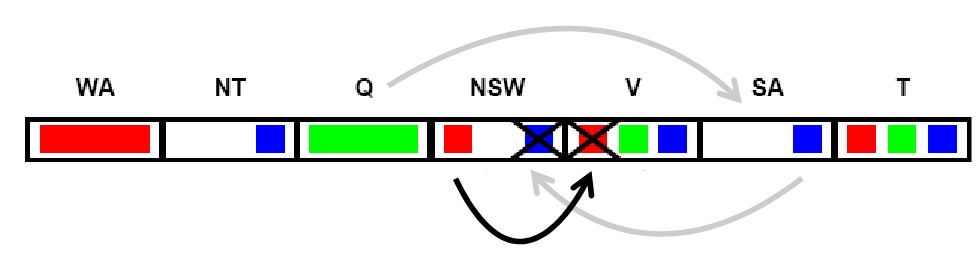
\includegraphics[width=0.6\textwidth]{Pics/05/ArcConsistency2.png}
\end{figure}

\begin{codebox}
    [AC-3 Algorithm]
    \begin{algorithm}[H]
        \SetKwFunction{acthree}{AC-3}
        \SetKwFunction{remfir}{remove\_first}
        \SetKwFunction{remincval}{remove\_inconsistent\_values}
        \SetKwFunction{neighbors}{get\_neighbors}
        \SetKwFunction{adddd}{add}
        \SetKwFunction{removee}{remove}
        \SetKwFunction{domaind}{get\_domain}
        \SetKwFunction{getarcs}{get\_all\_arcs}

        \Fn{\acthree{csp}}{
            queue = \getarcs{csp}\;
            \While{queue is not empty}{
                ($X_i,X_j$) = \remfir{queue}\;
                \If{\remincval{$X_i$, $X_j$}}{
                    \ForEach{$X_k$ in \neighbors{$X_i$}}{
                        queue.\adddd{$X_k$}\;
                    }
                }
            }
        }
        \Fn{\remincval{$X_i$, $X_j$}}{
            removed = false\;
            \ForEach{$x$ in \domaind{$X_i$}}{
                \If{no value $y$ in \domaind{$X_j$} satisfies \texttt{arc}($X_i, X_j$)}{
                    \domaind{$X_i$}.\removee{$x$}\;
                    removed = true\;
                }
            }
            \KwRet removed\;
        }
    \end{algorithm}
\end{codebox}

\subsubsection{Path Consistency}
Arc consistency is often sufficient to:
\begin{itemize}
    \item Solve the problem (all variable domains reduced to one value)
    \item Show that the problem cannot be solved (some domains empty)
\end{itemize}
but sometimes may not be enough, for example if theres always a consistent value in the neighboring region.

\defc{Path consistency} tightens the binary constraint by considering triples of values. 

A pair of variables $(X_i,X_j)$ is path-consistent with $X_m$ if
\begin{itemize}
    \item for every assignment that satisfies the constraint on the arc $(X_i, X_j)$
    \item there is an assignment that satisfies the constraints on the arcs $(X_i, X_m)$ and $(X_j, X_m)$
\end{itemize}

\subsubsection{k-Consistency}
k-Consistency is a generalization of path consistency. A set of k values need to be consistent. It may lead to a faster solution but checking for k-consistency is computationally expensive with exponential time in the worst case. 

In practice, arc consistency is most frequently used.

\subsubsection{Constrain Propagation \& Backtracking Search}
\defc{Basic Idea:}
Each time a variable is assigned, a constraint propagation algorithm is run in order to reduce the number of choice points in the search. This can improve the speed of backtracking search further. This algorithm can be implemented using Forward Checking or AC-3.

\newpage
\subsection{Local Search for CSPs}
\begin{minipage}
    [t]{0.5\textwidth}
    \textbf{Neccessary Modifications for CSPs:}
    \begin{itemize}
        \item work with complete states
        \item allow states with unsatisfied constraints
        \item operators reassign variable values
    \end{itemize}
\end{minipage}
\begin{minipage}
    [t]{0.5\textwidth}
    \textbf{Min-Conflicts Heuristic:}
    \begin{itemize}
        \item Randomly select a conflicted variable
        \item Choose the value that violates fewest constraints
        \item Hill climbing with h(n) = \# of violated constraints
    \end{itemize}
\end{minipage}

\textbf{Performance:}
\begin{itemize}
    \item Can solve randomly generated CSPs with a high probability
    \item Except in a narrow range $R = \dfrac{\text{\# of constraints}}{\text{\# of variables}}$
\end{itemize}

\subsection{Problem Decomposition}
Assume search space for a constraint satisfaction with \defc{n variables}, each of which can have \defc{d values} = $O(d^n)$

\defc{Basic Idea:}
Decompose the problem into subproblems with \defc{c variables} each
\begin{itemize}
    \item Each problem has complexity $O(d^c)$
    \item There are n/c problems $\rightarrow$ total complexity $O(n/c\cdot d^c)$
    \item Unconditional independence is rare
\end{itemize}

This can reduce the total complexity from exponential to linear, assuming c is constant.

\subsection{Tree-Structured CSPs}
A CSP is tree-structured if in the constraint graph any two variables are connected by a single path. Any tree structured CSP can be solved in linear time in the number of variables = $O(n\cdot d^2)$

\subsubsection{Linear Algorithm}
\begin{enumerate}
    \item Choose variable as root, order nodes so that parent always comes before its children (only one parent per node)
    \item For j = n downto 2
    \begin{itemize}
        \item Make the arc($X_i, X_{j}$) arc-consistent, calling \texttt{remove\_inconsistent\_value($X_i, X_{j}$)}
    \end{itemize}
    \item For i = 1 to n
    \begin{itemize}
        \item Assign to $X_i$ any value that is consistent with its parent
    \end{itemize}
\end{enumerate}

\begin{figure}
    [H]
    \centering
    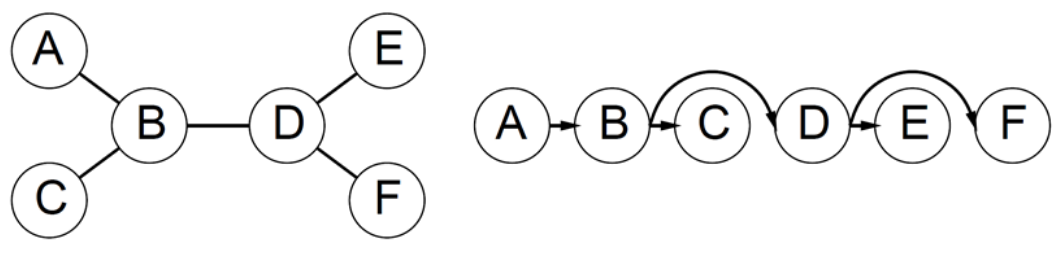
\includegraphics[width=0.6\textwidth]{Pics/05/LinearAlgorithmTree.png}
\end{figure}

\subsubsection{Nearly Tree-Structured Problems}
Tree structured problems are rare.

\textbf{Approaches for making them tree-structured:}
\begin{enumerate}
    \item \defc{Cutset Conditioning:}
    \begin{itemize}
        \item Removing nodes so that the remaining nodes form a tree
    \end{itemize}
    \item \defc{Collapsing nodes together:}
    \begin{itemize}
        \item Decompose the graph into a set of independent tree-shaped subproblems
    \end{itemize}
\end{enumerate}

\subsubsection*{Cutset Conditioning}
\begin{enumerate}
    \item Choose a subset S of the variables such that the constraint graph becomes a tree after removal of S (cycle cutset)
    \item Choose a consistent assignment of variables for S
    \item Remove from the remaining variables all values that are inconsistent with the variables of S
    \item Solve the CSP problem with the remainign variables
    \item If no solution: Choose different S in \textbf{2}
\end{enumerate}

\begin{figure}
    [H]
    \centering
    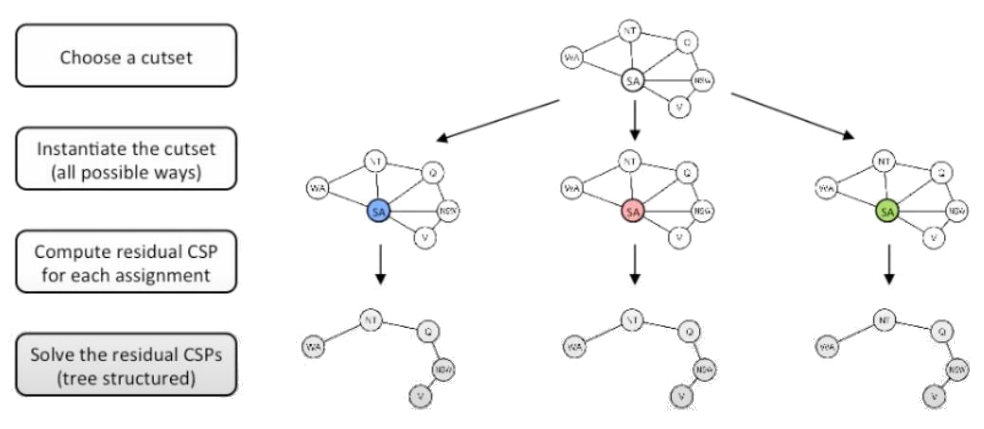
\includegraphics[width=0.6\textwidth]{Pics/05/CutsetConditioning.png}
\end{figure}
\end{document}